\documentclass[12pt]{article}

%
% Make a bigger page, but leave room for marginal notes.
%
\setlength{\topmargin}{-1.0 in}
\setlength{\oddsidemargin}{-0.5 in}
\setlength{\evensidemargin}{-0.5 in}
\setlength{\textwidth}{7.0 in}
\setlength{\textheight}{9.5 in}

\pagestyle{empty}

\usepackage{times}
\usepackage{mathtime}

\usepackage{graphicx}

\begin{document}

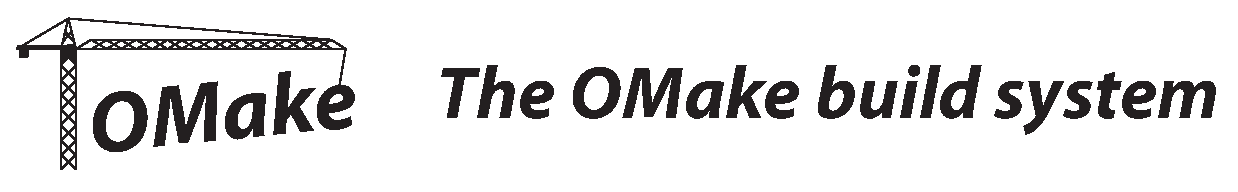
\includegraphics[scale=0.85]{omake}

OMake is a build system, similar to GNU make, but it support
hierarchical projects with automated dependency analysis, and the
language is {\bf functional}.  The home site for OMake is {\sf
http://omake.metaprl.org/}.

Features include:
\begin{itemize}
\item Support for large projects spanning several directories or
     directory hierarchies.

\item Comes with a default configuration file providing support for OCaml,
     C and LaTeX projects, or a mixture thereof.
     Often, a configuration file is as simple as a single line

\begin{verbatim}
        OCamlProgram(prog, foo bar baz)
\end{verbatim}

     which states that the program \verb+prog+ is built from the files
     \verb+foo.ml+, \verb+bar.ml+, and \verb+baz.ml+.

\item Fast, reliable, automated dependency analysis using MD5 digests.

\item Portability: omake provides a uniform interface on Win32 and
     on Unix systems including Linux and OSX.

\item Builtin functions that provide the most common features of programs
     like \verb+grep+, \verb+sed+, and \verb+awk+.  These are especially useful on Win32.

\item Full native support for rules that build several things at once.

\item Active filesystem monitoring, where the build automatically restarts
     whenever you modify a source file.  This can be very useful during
     the edit/compile cycle.

\item A companion command interpreter, \verb+osh+, that can be used interactively.
\end{itemize}

In the MetaPRL ({\sf http://www.metaprl.org}) and Mojave
({\sf http://mojave.caltech.edu}) projects we develop and maintain several
moderately large systems consisting of a mixture of OCaml, C, and
theorem proving code.  We developed OMake out of the need for a build
system that was simple, flexible, and reliable, especially for large
projects.

OMake preserves the syntax and rule definitions used in Makefiles,
making it easy to port your project to omake.  There is no need to
code in perl (cons), or Python (scons).  However, there are a few
things to keep in mind:

\begin{enumerate}
\item Indentation is significant, but tabs are not required.
\item The omake language is {\bf functional}: functions are first-class
      and there are no side-effects apart from I/O.
\item Scoping is dynamic.
\end{enumerate}

\noindent
OMake 0.9.2 is an alpha release.\\
Please report any comments and/or bugs to the mailing
list {\sf omake@metaprl.org}.
\vfill

\noindent
{\tiny Jason Hickey, {\sf jyh@cs.caltech.edu}}

\end{document}